\documentclass[xcolor={x11names, rgb, usenames, dvipsnames}]{beamer}
% Beamer loads xcolor by default. Do not load it a second time using \usepackage

\usepackage[francais, english]{babel}
\usepackage[T1]{fontenc}
\usepackage[utf8]{inputenc}
\usepackage{pgfplots}
\pgfplotsset{compat=1.12}
\usetikzlibrary{patterns}
\usepackage{graphicx}
\usepackage{hyperref}
\usepackage{amsmath}
\usepackage{amssymb}


\setbeamertemplate{bibliography item}{[\theenumiv]}

%\usetheme{Warsaw}
% \usetheme{Boadilla}
% \usetheme{Antibes}
\usetheme{CambridgeUS}
\usecolortheme{dolphin}
% \usetheme{Berlin}
% \usetheme{Madrid}
% \setbeamertemplate{footline}[frame number]


%http://tex.stackexchange.com/questions/160825/modifying-margins-for-one-slide
\newcommand\Wider[2][3em]{%
\makebox[\linewidth][c]{%
  \begin{minipage}{\dimexpr\textwidth+#1\relax}
  \raggedright#2
  \end{minipage}%
  }%
}




% http://tex.stackexchange.com/questions/116077/presentation-beamer-title-page
\makeatletter
\newcommand\titlegraphicii[1]{\def\inserttitlegraphicii{#1}}
\titlegraphicii{}
\setbeamertemplate{title page}
{
  \vbox{}
  \vspace{-2.5em}
   {\usebeamercolor[fg]{titlegraphic}\inserttitlegraphic\hfill\inserttitlegraphicii\par}
  \vskip2.5em
  \begin{centering}
    \begin{beamercolorbox}[sep=8pt,center]{institute}
      \usebeamerfont{institute}\insertinstitute
    \end{beamercolorbox}
    \begin{beamercolorbox}[sep=8pt,center]{title}
      \usebeamerfont{title}\inserttitle\par%
      \ifx\insertsubtitle\@empty%
      \else%
        \vskip0.25em%
        {\usebeamerfont{subtitle}\usebeamercolor[fg]{subtitle}\insertsubtitle\par}%
      \fi%     
    \end{beamercolorbox}%
    \vskip1em\par
    \begin{beamercolorbox}[sep=8pt,center]{date}
      \usebeamerfont{date}\insertdate
    \end{beamercolorbox}%\vskip0.5em
    \begin{beamercolorbox}[sep=8pt,center]{author}
      \usebeamerfont{author}\insertauthor
    \end{beamercolorbox}
  \end{centering}
  %\vfill
}
\makeatother

\author{Quentin Delhaye}
\title[Crypto using a Soc Platform]{Implementation of High-Level\\ Cryptographic Protocols using a SoC platform}
% \subtitle{}
\institute[ULB]{Université Libre de Bruxelles}
\date{June 24th, 2015}

\titlegraphic{
\includegraphics[width=1.5cm]{ulbnorm}}
\titlegraphicii{
\includegraphics[width=1.5cm]{logo-polytech-seul}}


%%%%%%%%%%%%%%%%%%%%%%%%
% data
%%%%%%%%%%%%%%%%%%%%%%%%
\def\temperaturedata{temperaturesOslo.txt}
\tikzstyle{maxmark} = [mark=*,mark options={color=red,scale=15}]
\tikzstyle{minmark} = [mark=*,mark options={color=blue,scale=15}]

% Lists
% \def\labelitemi{$\blacktriangleright$}

% \AtBeginSection[]
% {
%   \begin{frame}
%   \frametitle{Contents}
%   \tableofcontents[currentsection]
%   \end{frame}
% }


\begin{document}

\begin{frame}[plain, noframenumbering]
\titlepage
\end{frame}

\begin{frame}
	\frametitle{Contents}
	\tableofcontents[hideallsubsections]
	% \tableofcontents
\end{frame}


\section{Context}

\subsection{Objectives}
\begin{frame}
\frametitle{Objectives}
\begin{itemize}
	\item Real life use cases.
	\item Decrease CPU load.
	\item Improve performance.
\end{itemize}
\end{frame}








\section{Cryptographic protocols}
% \begin{frame}
% \frametitle{Contents}
% \tableofcontents[currentsection]
% \end{frame}

\begin{frame}
\frametitle{Cryptographic protocols}
\begin{description}
	\item[VPN]~\\
		\begin{itemize}
			\item TLS
			\item IPsec
		\end{itemize}
	\item[Schemes]~\\
		\begin{itemize}
			\item AES
			\item SHA-2
			\item Diffie-Hellman
			\item RSA
		\end{itemize}
\end{description}
\end{frame}



\section{Platform}
\begin{frame}
\frametitle{Contents}
\tableofcontents[%
	currentsection,
	sectionstyle=show/shaded,%Show the current section, shade the others
	subsectionstyle=show/show/hide,%Show the current subsection, show the other subsections of the same section, hide the other other subsections.
	]
\end{frame}


\subsection{Hardware}
\begin{frame}
\frametitle{SoCrates}
	\begin{figure}
	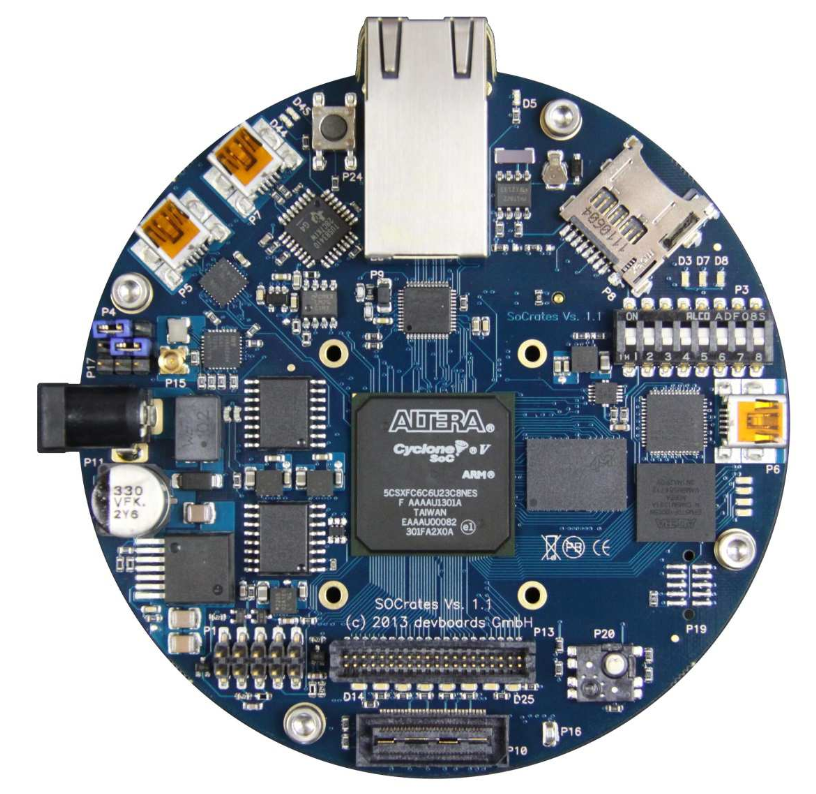
\includegraphics[height=4cm]{../socrates-photo.png}
	\end{figure}
	
	\begin{itemize}
		\item Dual core ARM Cortex A9 @ 800MHz
		\item Altera Cyclone V
		\item Gigabit Ethernet
	\end{itemize}
\end{frame}


\subsection{Operating System}
\begin{frame}
\frametitle{Linux structure}
	\begin{center}
	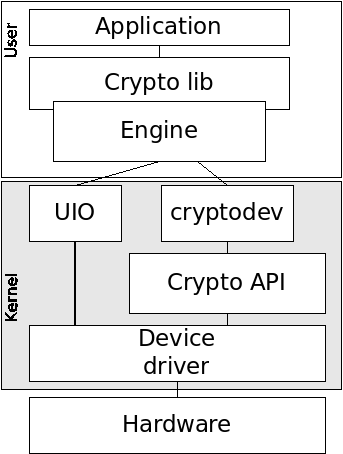
\includegraphics[height=7cm]{os-path-generic.png}
	\end{center}
\end{frame}


\begin{frame}
\frametitle{Linux structure (Cont'd)}
	\begin{center}
	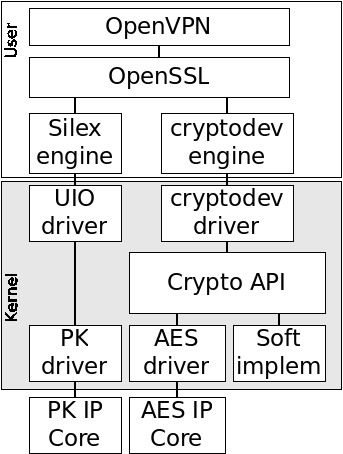
\includegraphics[height=7cm]{os-path-specific.png}
	\end{center}
\end{frame}





\section{Implementation}
\begin{frame}
\frametitle{Contents}
\tableofcontents[%
	currentsection,
	sectionstyle=show/shaded,
	subsectionstyle=show/show/hide,
	]
\end{frame}

\subsection{OpenVPN}
\begin{frame}
\frametitle{OpenVPN}
	\begin{figure}
	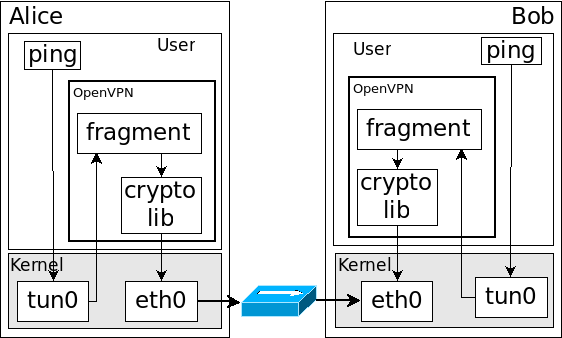
\includegraphics[height=6cm]{openvpn-transfer.png}
	\end{figure}
\end{frame}

\subsection{IPsec}
\begin{frame}
\frametitle{IPsec}
	\begin{figure}
	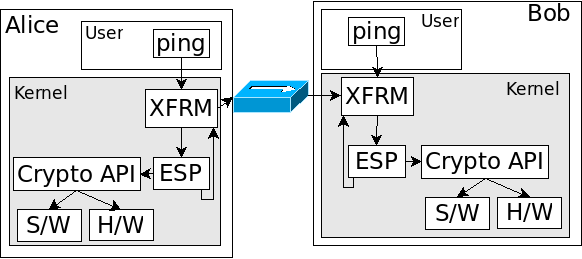
\includegraphics[height=5cm]{ipsec-transfer.png}
	\end{figure}
\end{frame}




\section{Results}
\begin{frame}
\frametitle{Contents}
\tableofcontents[%
	currentsection,
	sectionstyle=show/shaded,
	subsectionstyle=show/show/hide,
	]
\end{frame}


\subsection{TLS connections}

\begin{frame}
\frametitle{TLS connections -- Context}
\begin{center}
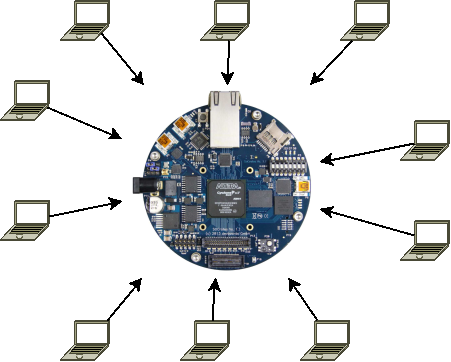
\includegraphics[height=3cm]{tls-bench.png}
\end{center}
\begin{itemize}
	\item 1 server, 10 clients
	\item 1-second connections
	\item RSA-1024/2048/4096
	\item OpenVPN
\end{itemize}
\end{frame}

\begin{frame}
\frametitle{TLS connections -- OpenVPN}
\Wider[1em]{%
	\begin{minipage}[c]{.48\linewidth}
		\begin{tikzpicture}
		%%%%%%%%%%%%%%%%%%%%%%%%
% throughput
%%%%%%%%%%%%%%%%%%%%%%%%
\begin{axis}[
        % title = {FTP transfer inside an IPSec tunnel},
        width  = \textwidth,
        height = 0.65\paperheight,
        major x tick style = transparent,
        xbar=2pt,
        bar width=8pt,
        % enlarge x limits={abs=1},
        xmajorgrids = true,
        xlabel = {Connections per minute},
        ylabel = {},
        ylabel near ticks,
        yticklabel pos=right,
        xmin=0, xmax=600,
        xtick={0,100,200,300,400,500},
        symbolic y coords={RSA-1024, RSA-2048, RSA-4096},
        ytick = data,
        scaled x ticks = false,%Disable the *10^4 exponent applied to all y axis markings.
        legend style={at={(1.3,-0.1)}, anchor=north,legend columns=1},
        % enlarge x limits=0.1,
    ]

\addplot[style={black,fill=ForestGreen,mark=none}, nodes near coords={\pgfmathfloatifflags{\pgfplotspointmeta}{0}{}{\pgfmathprintnumber{\pgfplotspointmeta}}}]
    coordinates {
        (445.4,RSA-1024)
        (155.6,RSA-2048)
        (19.6,RSA-4096)
    };
    \label{soft-tp}

\addplot[style={black,fill=BrickRed,mark=none}, nodes near coords={\pgfmathfloatifflags{\pgfplotspointmeta}{0}{}{\pgfmathprintnumber{\pgfplotspointmeta}}}]
    coordinates {
        (509.3,RSA-1024)
        (420.9,RSA-2048)
        (115.5,RSA-4096)
    };
    \label{ba411e-tp}
\legend{\small software, H/W}
\end{axis}
		\end{tikzpicture}
	\end{minipage} \hfill
	\begin{minipage}[c]{.44\linewidth}
		\begin{tikzpicture}
		%%%%%%%%%%%%%%%%%%%%%%%%
% throughput
%%%%%%%%%%%%%%%%%%%%%%%%
\begin{axis}[
        % title = {FTP transfer inside an IPSec tunnel},
        width  = \textwidth,
        height = 0.65\paperheight,
        major x tick style = transparent,
        xbar=2pt,
        bar width=8pt,
        % enlarge x limits={abs=1},
        xmajorgrids = true,
        xlabel = {CPU usage},
        ylabel = {},
        % ylabel near ticks,
        % yticklabel pos=right,
        xmin=0, xmax=115,
        xtick={50, 100},
        symbolic y coords={RSA-1024, RSA-2048, RSA-4096},
        ytick = data,
        ymajorticks=false,
        scaled x ticks = false,%Disable the *10^4 exponent applied to all y axis markings.
        legend style={at={(0.5,-0.15)}, anchor=north,legend columns=4},
        % enlarge x limits=0.1,
    ]

\addplot[style={black,fill=LimeGreen,postaction={pattern=north east lines},mark=none}, nodes near coords={\pgfmathfloatifflags{\pgfplotspointmeta}{0}{}{\pgfmathprintnumber{\pgfplotspointmeta}}}]
    coordinates {
        (40.32,RSA-1024)
        (92.14,RSA-2048)
        (81.97,RSA-4096)
    };
    \label{software}

\addplot[style={black,fill=RedOrange,postaction={pattern=north east lines},mark=none}, nodes near coords={\pgfmathfloatifflags{\pgfplotspointmeta}{0}{}{\pgfmathprintnumber{\pgfplotspointmeta}}}]
    coordinates {
        (13.29,RSA-1024)
        (4.82,RSA-2048)
        (4.78,RSA-4096)
    };
    \label{ba414e}
% \legend{software, ba411e, out-of-tunnel, inside tunnel}
\end{axis}
		\end{tikzpicture}
		\vspace{0.5cm}
	\end{minipage}
}
\end{frame}


\subsection{File transfer}

\begin{frame}
\frametitle{File transfer -- Context}
\begin{center}
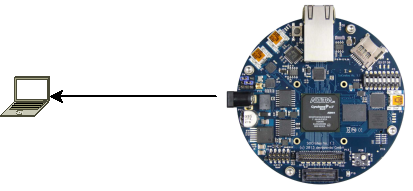
\includegraphics[height=3cm]{ftp-bench.png}
\end{center}
\begin{itemize}
	\item 128MB file
	\item AES-256-CBC/SHA-256
	\item OpenVPN/IPsec
\end{itemize}
\end{frame}

\begin{frame}
\frametitle{File transfer -- OpenVPN}
\Wider[1em]{%
	\begin{minipage}[c]{.48\linewidth}
		\begin{tikzpicture}
		%%%%%%%%%%%%%%%%%%%%%%%%
% throughput
%%%%%%%%%%%%%%%%%%%%%%%%
\begin{axis}[
        % title = {FTP transfer inside an IPSec tunnel},
        width  = \textwidth,
        height = 0.75\paperheight,
        major x tick style = transparent,
        xbar=2pt,
        bar width=8pt,
        % enlarge x limits={abs=1},
        xmajorgrids = true,
        xlabel = {Throughput [MB/s]},
        ylabel = {},
        ylabel near ticks,
        yticklabel pos=right,
        xmin=0, xmax=15,
        symbolic y coords={cipher null, aes:none, aes:sha},
        ytick = data,
        scaled x ticks = false,%Disable the *10^4 exponent applied to all y axis markings.
        legend style={at={(1.3,-0.1)}, anchor=north,legend columns=2},
        % enlarge x limits=0.1,
    ]

\addplot[style={black,fill=ForestGreen,mark=none}, nodes near coords={\pgfmathfloatifflags{\pgfplotspointmeta}{0}{}{\pgfmathprintnumber{\pgfplotspointmeta}}}]
    coordinates {
        (0,cipher null)
        (4.78,aes:none)
        (3.87,aes:sha)
    };
    \label{software}

\addplot[style={black,fill=black,mark=none}, nodes near coords={\pgfmathfloatifflags{\pgfplotspointmeta}{0}{}{\pgfmathprintnumber{\pgfplotspointmeta}}}]
    coordinates {
        (11.39,cipher null)
        (0,aes:none)
        (0,aes:sha)
    };
    \label{out-of-tunnel}%"tp" for "throughput"

\addplot[style={black,fill=BrickRed,mark=none}, nodes near coords={\pgfmathfloatifflags{\pgfplotspointmeta}{0}{}{\pgfmathprintnumber{\pgfplotspointmeta}}}]
    coordinates {
        (0,cipher null)
        (3.35,aes:none)
        (2.84,aes:sha)
    };
    \label{ba411e}

\addplot[style={black,fill=MidnightBlue,mark=none}, nodes near coords={\pgfmathfloatifflags{\pgfplotspointmeta}{0}{}{\pgfmathprintnumber{\pgfplotspointmeta}}}]
    coordinates {
        (5.18,cipher null)
        (0,aes:none)
        (0,aes:sha)
    };
    \label{inside tunnel}
\legend{\small software, raw, ba411e, OpenVPN}
\end{axis}
		\end{tikzpicture}
	\end{minipage} \hfill
	\begin{minipage}[c]{.44\linewidth}
		\begin{tikzpicture}
		%%%%%%%%%%%%%%%%%%%%%%%%
% throughput
%%%%%%%%%%%%%%%%%%%%%%%%
\begin{axis}[
        % title = {FTP transfer inside an IPSec tunnel},
        width  = \textwidth,
        height = 0.75\paperheight,
        major x tick style = transparent,
        xbar=2pt,
        bar width=8pt,
        % enlarge x limits={abs=1},
        xmajorgrids = true,
        xlabel = {CPU usage},
        ylabel = {},
        % ylabel near ticks,
        % yticklabel pos=right,
        xmin=0, xmax=115,
        xtick={50, 100},
        symbolic y coords={cipher null, aes:none, aes:sha},
        ytick = data,
        ymajorticks=false,
        scaled x ticks = false,%Disable the *10^4 exponent applied to all y axis markings.
        legend style={at={(0.5,-0.15)}, anchor=north,legend columns=4},
        % enlarge x limits=0.1,
    ]

\addplot[style={black,fill=LimeGreen,postaction={pattern=north east lines},mark=none}, nodes near coords={\pgfmathfloatifflags{\pgfplotspointmeta}{0}{}{\pgfmathprintnumber{\pgfplotspointmeta}}}]
    coordinates {
        (0,cipher null)
        (76.60,aes:none)
        (76.03,aes:sha)
    };
    \label{software-cpu}

\addplot[style={black,fill=gray,postaction={pattern=north east lines},mark=none}, nodes near coords={\pgfmathfloatifflags{\pgfplotspointmeta}{0}{}{\pgfmathprintnumber{\pgfplotspointmeta}}}]
    coordinates {
        (7.16,cipher null)
        (0,aes:none)
        (0,aes:sha)
    };
    \label{out-of-tunnel-cpu}%"oot" for "out of tunnel"

\addplot[style={black,fill=RedOrange,postaction={pattern=north east lines},mark=none}, nodes near coords={\pgfmathfloatifflags{\pgfplotspointmeta}{0}{}{\pgfmathprintnumber{\pgfplotspointmeta}}}]
    coordinates {
        (0,cipher null)
        (83.74,aes:none)
        (80.89,aes:sha)
    };
    \label{ba411e-cpu}

\addplot[style={black,fill=NavyBlue,postaction={pattern=north east lines},mark=none}, nodes near coords={\pgfmathfloatifflags{\pgfplotspointmeta}{0}{}{\pgfmathprintnumber{\pgfplotspointmeta}}}]
    coordinates {
        (42.60,cipher null)
        (0,aes:none)
        (0,aes:sha)
    };
    \label{inside tunnel-cpu}%"it" for "in tunnel"
% \legend{software, ba411e, out-of-tunnel, inside tunnel}
\end{axis}
		\end{tikzpicture}
		\vspace{0.7cm}
	\end{minipage}
}
\end{frame}


\begin{frame}
\frametitle{File transfer -- IPsec}
\Wider[1em]{%
	\begin{minipage}[c]{.48\linewidth}
		\begin{tikzpicture}
		%%%%%%%%%%%%%%%%%%%%%%%%
% throughput
%%%%%%%%%%%%%%%%%%%%%%%%
\begin{axis}[
        % title = {FTP transfer inside an IPSec tunnel},
        width  = \textwidth,
        height = 0.75\paperheight,
        major x tick style = transparent,
        xbar=2pt,
        bar width=8pt,
        % enlarge x limits={abs=1},
        xmajorgrids = true,
        xlabel = {Throughput [MB/s]},
        ylabel = {},
        ylabel near ticks,
        yticklabel pos=right,
        xmin=0, xmax=15,
        symbolic y coords={cipher null, aes:none, aes:sha},
        ytick = data,
        scaled x ticks = false,%Disable the *10^4 exponent applied to all y axis markings.
        legend style={at={(1.3,-0.1)}, anchor=north,legend columns=2},
        % enlarge x limits=0.1,
    ]

\addplot[style={black,fill=ForestGreen,mark=none}, nodes near coords={\pgfmathfloatifflags{\pgfplotspointmeta}{0}{}{\pgfmathprintnumber{\pgfplotspointmeta}}}]
    coordinates {
        (0,cipher null)
        (8.83,aes:none)
        (6.47,aes:sha)
    };

\addplot[style={black,fill=black,mark=none}, nodes near coords={\pgfmathfloatifflags{\pgfplotspointmeta}{0}{}{\pgfmathprintnumber{\pgfplotspointmeta}}}]
    coordinates {
        (11.39,cipher null)
        (0,aes:none)
        (0,aes:sha)
    };

\addplot[style={black,fill=BrickRed,mark=none}, nodes near coords={\pgfmathfloatifflags{\pgfplotspointmeta}{0}{}{\pgfmathprintnumber{\pgfplotspointmeta}}}]
    coordinates {
        (0,cipher null)
        (8.52,aes:none)
        (5.80,aes:sha)
    };

\addplot[style={black,fill=MidnightBlue,mark=none}, nodes near coords={\pgfmathfloatifflags{\pgfplotspointmeta}{0}{}{\pgfmathprintnumber{\pgfplotspointmeta}}}]
    coordinates {
        (10.21,cipher null)
        (0,aes:none)
        (0,aes:sha)
    };
\legend{\small software, raw, H/W, IPsec}
\end{axis}
		\end{tikzpicture}
	\end{minipage} \hfill
	\begin{minipage}[c]{.44\linewidth}
		\begin{tikzpicture}
		%%%%%%%%%%%%%%%%%%%%%%%%
% throughput
%%%%%%%%%%%%%%%%%%%%%%%%
\begin{axis}[
        % title = {FTP transfer inside an IPSec tunnel},
        width  = \textwidth,
        height = 0.75\paperheight,
        major x tick style = transparent,
        xbar=2pt,
        bar width=8pt,
        % enlarge x limits={abs=1},
        xmajorgrids = true,
        xlabel = {CPU usage},
        ylabel = {},
        % ylabel near ticks,
        % yticklabel pos=right,
        xmin=0, xmax=100,
        symbolic y coords={cipher null, aes:none, aes:sha},
        ytick = data,
        ymajorticks=false,
        scaled x ticks = false,%Disable the *10^4 exponent applied to all y axis markings.
        legend style={at={(0.5,-0.15)}, anchor=north,legend columns=4},
        % enlarge x limits=0.1,
    ]

\addplot[style={black,fill=LimeGreen,postaction={pattern=north east lines},mark=none}, nodes near coords={\pgfmathfloatifflags{\pgfplotspointmeta}{0}{}{\pgfmathprintnumber{\pgfplotspointmeta}}}]
    coordinates {
        (0,cipher null)
        (63.74,aes:none)
        (74.64,aes:sha)
    };
    \label{software-cpu}

\addplot[style={black,fill=gray,postaction={pattern=north east lines},mark=none}, nodes near coords={\pgfmathfloatifflags{\pgfplotspointmeta}{0}{}{\pgfmathprintnumber{\pgfplotspointmeta}}}]
    coordinates {
        (7.16,cipher null)
        (0,aes:none)
        (0,aes:sha)
    };
    \label{out-of-tunnel-cpu}%"oot" for "out of tunnel"

\addplot[style={black,fill=RedOrange,postaction={pattern=north east lines},mark=none}, nodes near coords={\pgfmathfloatifflags{\pgfplotspointmeta}{0}{}{\pgfmathprintnumber{\pgfplotspointmeta}}}]
    coordinates {
        (0,cipher null)
        (14.87,aes:none)
        (17.25,aes:sha)
    };
    \label{ba411e-cpu}

\addplot[style={black,fill=NavyBlue,postaction={pattern=north east lines},mark=none}, nodes near coords={\pgfmathfloatifflags{\pgfplotspointmeta}{0}{}{\pgfmathprintnumber{\pgfplotspointmeta}}}]
    coordinates {
        (14.68,cipher null)
        (0,aes:none)
        (0,aes:sha)
    };
    \label{inside tunnel-cpu}%"it" for "in tunnel"
% \legend{software, ba411e, out-of-tunnel, inside tunnel}
\end{axis}
		\end{tikzpicture}
		\vspace{0.7cm}
	\end{minipage}
}
\end{frame}





\section{Conclusion}

\begin{frame}
\frametitle{Conclusion}
\begin{description}
	\item[TLS connections]~\\
		\begin{itemize}
			\item 589\% connections
			\item 5\% the CPU usage
		\end{itemize}
	\item[File transfer]~\\
		\begin{itemize}
			\item Drop OpenVPN
			\item 89\% performance
			\item 23\% the CPU usage
		\end{itemize}
\end{description}
\end{frame}


\begin{frame}
\frametitle{Conclusion}
\begin{itemize}
	\item Ongoing development
\end{itemize}

\end{frame}



% %%%%%%%%%%%%%%%%%%%%%%%%%%%%%%%%%%%%%%%%%%%%
% \section*{References}
% %%%%%%%%%%%%%%%%%%%%%%%%%%%%%%%%%%%%%%%%%%%%

% \nocite*{}
% \bibliographystyle{plain}
% \bibliography{bibliography}

\end{document}
